\documentclass{article}
\usepackage{pdfpages}
\usepackage{graphicx}  % For PNG
\usepackage[left=2cm, right=2cm, top=2cm]{geometry}
\usepackage{minted}
% Give Table of Contents Hyperlinks
\usepackage{hyperref}
\hypersetup{
    colorlinks,
    citecolor=black,
    filecolor=black,
    linkcolor=black,
    urlcolor=blue
}
\pagenumbering{gobble}
% \pagenumbering{roman} % set the numbering style to lowercase letter

\title{\textbf{Homework 4}}

\author{MacMillan, Kyle}
\date{October 19, 2018}

\begin{document}


\addcontentsline{toc}{section}{Title}
\maketitle

\newpage
\tableofcontents
\addcontentsline{toc}{section}{Table of Contents}

\pagenumbering{roman}   % Set TOC page numbering to lowercase roman numerals



%%%%%%%%%%%%%%%%%%%%%%%%%%%% INTRO SECTION %%%%%%%%%%%%%%%%%%%%%%%%%%%%
\newpage
\hypersetup{
    colorlinks,
    citecolor=blue,
    filecolor=black,
    linkcolor=blue,
    urlcolor=blue
}
\pagenumbering{arabic}  % Set content page numbering to arabic numerals

\setcounter{page}{1}
\newpage
\section{\textbf{Problem 9}}
\subsection{Problem 9.1}
Figure \ref{fig:9.1} shows the required plot. The robot location is:\\
$x = 803.84497$\\
$y = 485.52026$\\
$z = 517.26977$\\
With an error of $E = 2720.65$


\begin{figure}[h]
    \centering
    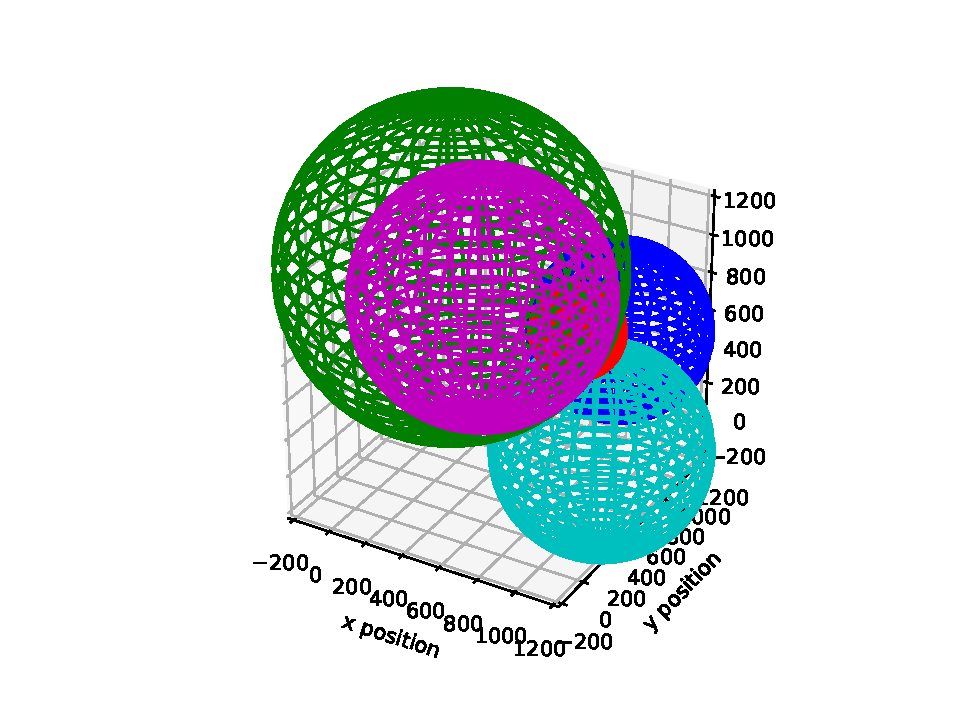
\includegraphics[pages=1]{problem9-1}
    \caption{Problem 9.1}
    \label{fig:9.1}
\end{figure}

\subsection{Problem 9.2}
\noindent $\lambda = c * 10 MHz$\\
$\lambda = 30\ meters$\\


Assuming phase shift $\theta = 10$ we can plug that into our formula to get

$$D' = L + \frac{\theta}{2\pi}\lambda$$
Therefore $D = \frac{D'}{2} = 0.833333333 + 15k$ where $k$ denotes an integer 
interval. We make the assumption that L is arbitrarily small compared to the 
distance travel and is therefore set to $0$. If the system has noise we will 
have to identify a range for $\frac{D'}{2}$, in this case it's $0.825\ to\ 
0.841666667 + 15k$. In order to differentiate between 20 and 250 meters we would 
need a second system at a $\lambda$ multiple that doesn't overlap before a 
distance of 250 meters.

\section{\textbf{Problem 10}}
\subsection{Problem 10.1}
asdf

\subsection{Probelm 10.2}
asdf

\end{document}
